\subsection{Numerical model}

The 0-D imposed-pressure reactor (IPR) model of Omnisoot~\citep{adib2026omnisoot} was used to simulate CB formation coupled with chemical kinetics during the pyrolysis process under post-reflected-shock conditions in the shock tube. IPR incorporates a sectional population balance model (SPBM) to describe the evolving size distribution of CB agglomerates by tracking the number of agglomerates, $N_{agg}$, primary particles, $N_{pri}$, total carbon, $C_{tot}$, and hydrogen content, $H_{tot}$.

The measured pressure trace was filtered to reduce noise and fluctuations, and then imposed on the model. The measured pressure remains within 10\% of the initial value until 2~ms for all tests. Fig.~\ref{fig:ptfv_pressure_type}a highlights the deviation of the (filtered) pressure time history from the initial pressure of P$_5$=4.30~atm at T$_5$=1984~K. The pressure starts to rise at $\approx$2.2~ms, reaches its peak at $\approx$3.1~ms, and drops towards the end of the test time due to the arrival of the expansion wave. Fig.~\ref{fig:ptfv_pressure_type}b shows a similar deviation in the predicted temperature. The analysis of species mole fractions showed that the imposed pressure results in lower CH$_4$ conversion and C$_2$H$_2$ yield, thereby reducing PAH formation and CB inception flux. As shown in Fig.~\ref{fig:ptfv_pressure_type}c, $f_v$ values predicted using constant and imposed pressure are close until 3.9~ms, but the discrepancy grows after that, where only the simulation with the imposed pressure captures the experimental time trends.


\begin{figure}[!t]
	\centering
	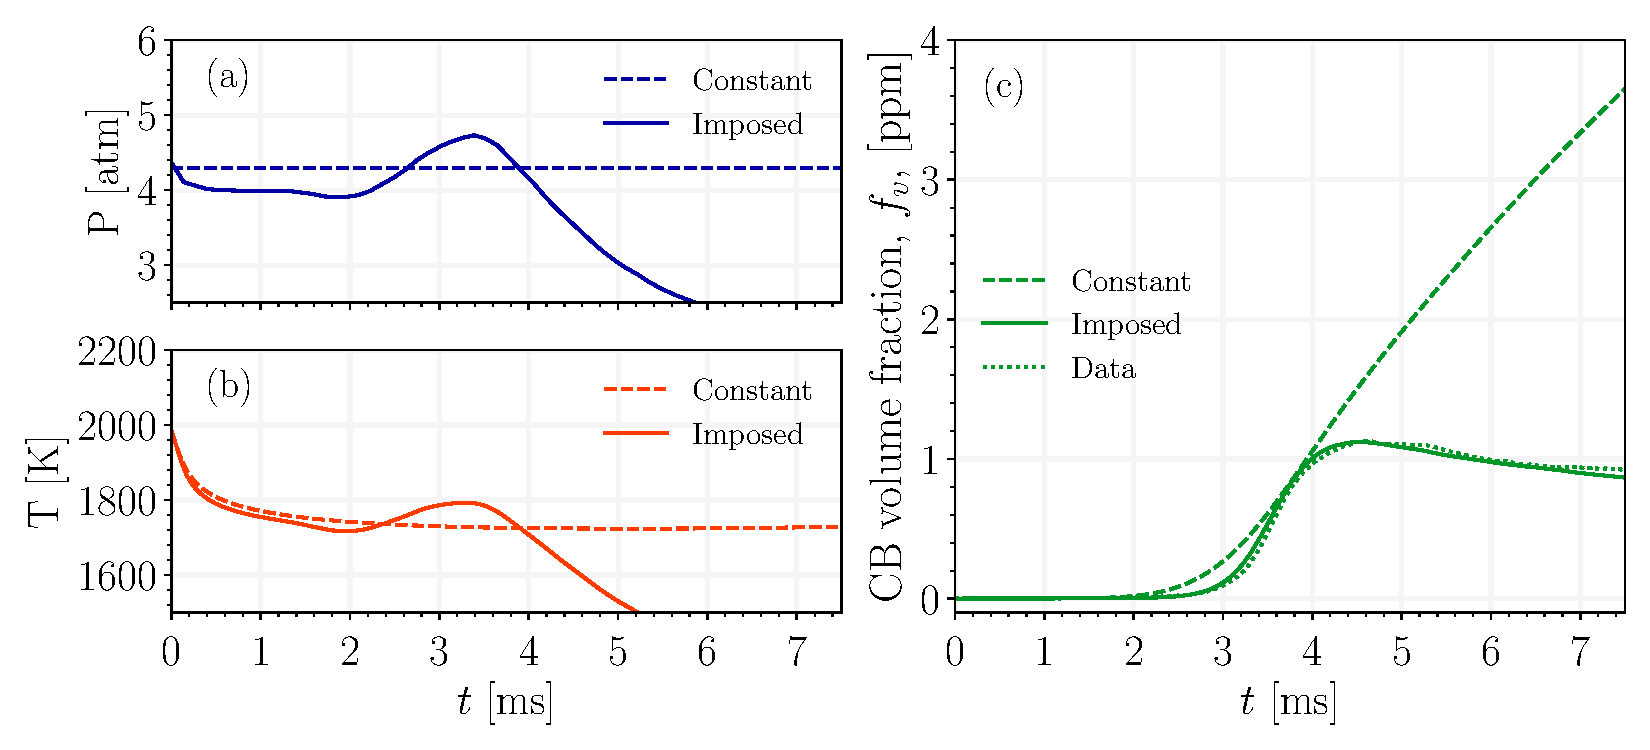
\includegraphics[width=1\textwidth]{Figures/Results/Paper3/PTfv_pressure_type.pdf}
	\caption{The comparison of (a) pressure (b) temperature (c) CB volume fraction for simulations with constant and imposed pressure trace at T$_5$=1984~K.}
	\label{fig:ptfv_pressure_type} 
\end{figure}

Soot precursors considered in this study include naphthalene (A2), phenanthrene (A3), pyrene (A4), acenaphthylene (A2R5), acephenanthrylene (A3R5), and cyclopentapyrene (A4R5), due to extensive support in the literature for their role in the initial steps of CB formation~\citep{mercier2019dimers,martin2019reactivity}. The E-Bridge Modified model is used to describe the dimerization and adsorption of precursors that contribute to CB inception and surface growth, respectively. The general formulation of the model is based on the inception model proposed by Frenklach and Mebel~\citep{frenklach2020mechanism}, with some modifications detailed in~\citep{adib2026omnisoot}. Two scaling factors, $\eta_{inc}$ and $\eta_{ads}$, between 0 and 1 are used to adjust the inception and PAH adsorption rates, respectively~\citep{adib2026omnisoot}.

The surface growth is described by the H-abstraction-$\mathrm{C_2H_2}$/Carbon-addition (HACA) scheme~\citep{appel2000kinetic}, but the surface density of hydrogenated sites, $\chi_{soot{\text-}H}$, is dynamically calculated as the ratio of hydrogen content to the surface area of agglomerates, i.e., $\chi_{soot{\text-}H}=H_{tot}/A_{tot}$~\citep{blanquart2009analyzing}. An Arrhenius equation is used to account for the loss of hydrogen by the carbonization of CB particles as~\citep{basile2002coagulation}:

\begin{equation}
	k_{carb}=
	A_{carb}\cdot \mathrm{exp}(\frac{-E_{carb}}{RT}),
	\label{eqn:k_carb}
\end{equation}

\begin{equation}
	\left(\frac{\mathrm{d}H_{tot}}{\mathrm{d}t}\right)_{\mathrm{carb}}=
	-k_{carb}\cdot H_{tot},
	\label{eqn:carb_rate}
\end{equation}

\noindent where $A_{carb}$ and $E_{carb}$ are the exponential prefactor and activation energy for carbonization, respectively. $H_{tot}/A_{tot}$ depends on the relative contributions of PAH adsorption and HACA, and the carbonization rate. The comparison of $\chi_{soot{\text-}H}$ with its nominal value of $2.3\times10^{19}$~sites/$m^2$ used in the original HACA formulation~\citep{frenklach1991detailed} shows that the dynamic method strongly depends on the temperature time history, and it predicts an overall larger number of reaction sites for T$_5$$<$2300~K (Fig.~\ref{fig:chi_soot_all_cases}).
